\documentclass[10pt,aspectratio=169]{beamer}
% Packages
\usepackage{mathabx}
\usepackage{xcolor}
\usepackage{amsmath}
\usepackage{mathtools}
\usepackage{standalone}
\usepackage{mhchem}
\usepackage{textpos}
\usepackage{graphicx}
\usepackage{wrapfig}
\graphicspath{{images}}

% Configure template
\setbeamertemplate{navigation symbols}{}

% Theme
\usetheme[progressbar=frametitle]{metropolis}
\setbeamertemplate{caption}[numbered]
\setbeamersize{text margin left=5mm,text margin right=5mm}

% Title page details: 
\title{Scientific Computing: Molecular dynamics}
\subtitle{Problemsheet 2}
\author{Jimin Kim, Christian Nix, Noah Schlenker}
\date{17. Mai 2024}
\institute{Technical University of Munich}

\begin{document}

% Title page frame
\maketitle

\addtobeamertemplate{frametitle}{}{
\begin{textblock*}{100mm} (.945\textwidth,-.85cm)

\includegraphics[scale=0.14]{../template/res/tum_logo.png}
\end{textblock*}}

% Outline frame
\begin{frame}{Outline}
    \tableofcontents
\end{frame}

%Slides for Unit tests
\section{Unit Tests}

\begin{frame}
    \frametitle{Google test for general testing}

        Integration of \emph{gtest} via CMake after checking presence in system

    \begin{figure}[H]
        
\includegraphics[width=\textwidth]{res/gtest3.png}
    \end{figure}


\end{frame}

\begin{frame}
    \frametitle{Google test for general testing}

        Handling src files as a library so that tests can be executed separately

    \begin{figure}[H]
        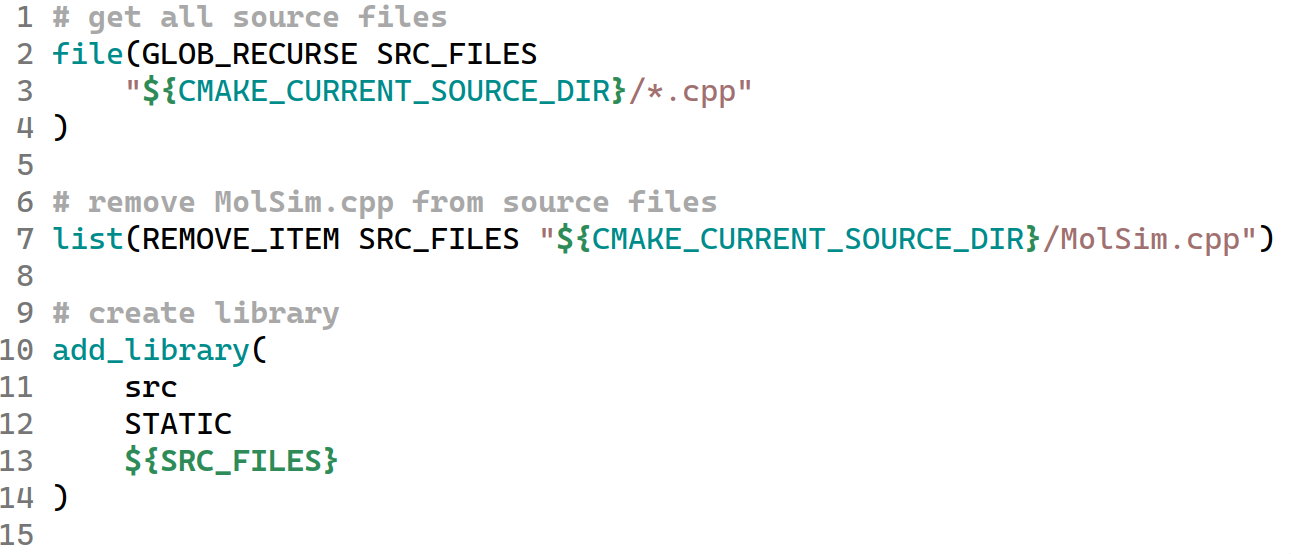
\includegraphics[width=\textwidth]{res/gtest1.png}
    \end{figure}


\end{frame}

\begin{frame}
    \frametitle{Google test for general testing}

        Handling src files as a library so that tests can be executed separately

    Linking with MolSim:
    \begin{figure}[H]
        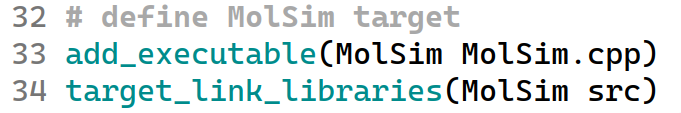
\includegraphics[width=0.5\textwidth]{res/gtest2.png}
    \end{figure}

    Linking with tests:
    \begin{figure}[H]
        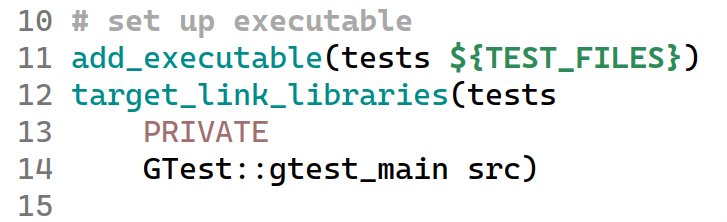
\includegraphics[width=0.5\textwidth]{res/gtest4.png}
    \end{figure}

\end{frame}



%Slides for CI
\section{Continuous Integration}

\begin{frame}
    \frametitle{Docker and act}

    \begin{itemize}
        \item Not much to mention: CI realization through Docker and 'nektos/act'
        \item Branch protection rules on \emph{master} and \emph{assignment*} branches
    \end{itemize}

\end{frame}

%Slides for spdlog
\section{Spdlog}

\begin{frame}
    \frametitle{spdlog functions vs macros}

    \begin{itemize}
        \item Incorporation using CMake module, including pre-fetch check for availability
        \item Macro benefits: Compile-time and run-time benefits
        \item Function benefits: type safety
        \item Run-time adjustment of log levels $\Rightarrow$ Compile-time benefits of macros not relevant
        \item Current project status undergoes frequent changes $\Rightarrow $safety preferred
    \end{itemize}
    \bigskip

    $\Rightarrow$ Log-level can be specified by user with option \texttt{-l}

\end{frame}




\section{Program Frame}

\begin{frame}
    \frametitle{UML model}


    \begin{figure}[H]
        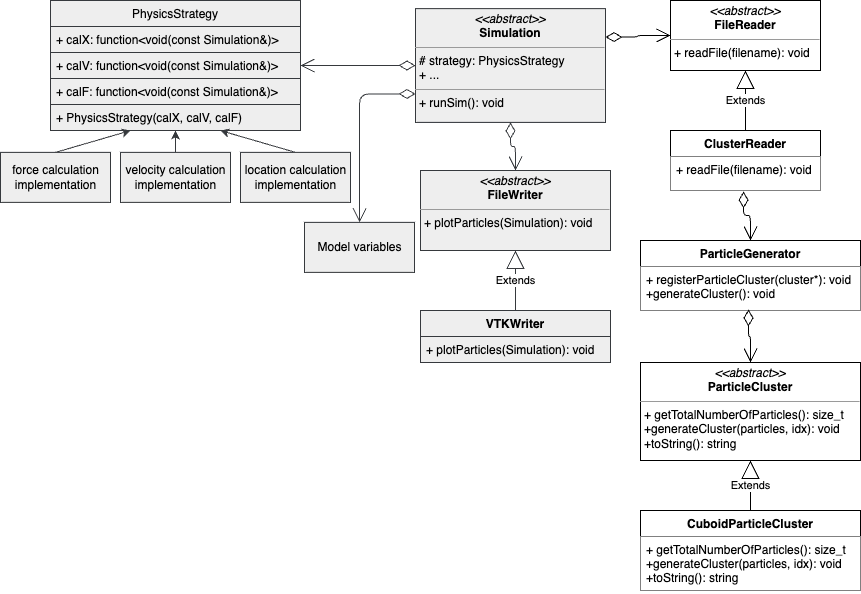
\includegraphics[width=0.72\textwidth]{res/UML.png}
    \end{figure}


\end{frame}

\section{Particle Generator}

\begin{frame}
    \frametitle{Abstracting Particle Clusters for simple Particle Generator}
    
    Particle clusters describe a collection of particles in a predefined structure

    \begin{itemize}
        \item \emph{ParticleCluster} is an abstract class requiring child classes to implement three methods:
        \begin{enumerate}
            \item (i) \emph{getTotalNumberOfParticles} $\rightarrow$ Returns the number of particles in the cluster
            \item (ii) \emph{generateCluster} $\rightarrow$ insert all particles into the passed particles vector
            \item (iii) \emph{toString} $\rightarrow$ Stringify for logging
        \end{enumerate}  
        \item We implemented a child class \emph{CuboidParticleCluster} which will generate a cluster as described on the problem sheet
        \item[] \!\!\!\!\!\!\!\!\! \textcolor{orange}{$\Rightarrow$} Abstraction allows for easy extension $\rightarrow$ "falling drop" sounds as if spherical clusters will become important
    \end{itemize}

    \begin{itemize}
        \item The \emph{ParticleGenerator} class has two methods to generate clusters of particles
        \begin{enumerate}
            \item \emph{registerCluster} $\rightarrow$ Add unique pointer to \emph{ParticleCluster} onto a vector 
            \item \emph{generateClusters} $\rightarrow$ Call \emph{generateCluster} on every registered \emph{ParticleCluster}
        \end{enumerate}
        \item[] \!\!\!\!\!\!\!\!\! \textcolor{orange}{$\Rightarrow$} Registering clusters first allows to know the total number of particles $\rightarrow$ allocate \textbf{one} vector 
    \end{itemize}

\end{frame}
\section{Lennard-Jones Forces}

\begin{frame}
    \frametitle{Rearraning formula to avoid unnecessary calculations}
    
    Let's start from the given formula and extract constant terms:

    \begin{align}
        F_{i,j} &= -\frac{\epsilon \cdot 24}{(||x_i-x_j||_2)^2} \left( \left( \frac{\sigma}{||x_i-x_j||_2} \right) ^6 - 2 \left( \frac{\sigma}{||x_i-x_j||_2} \right) ^{12} \right) (x_i-x_j) \\
                &= \frac{-\epsilon \cdot 24}{(||x_i-x_j||_2)^2} \left(  \frac{\sigma ^6 }{||x_i-x_j||_2 ^6 } + \frac{-2 \cdot \sigma^{12}}{||x_i-x_j||_2^{12}}  \right) (x_i-x_j)
    \end{align}

    Let $-\epsilon \cdot 24 =: \alpha$, $\sigma ^6 =: \beta$, and $-2 \cdot \sigma^{12} =: \gamma$ $\Rightarrow$ calculate once upon initialization of Lennard-Jones simulation \\
    Further, let $x_i-x_j =: \delta \in \mathbb{R}^3$

    \begin{align}
        F_{i,j} &= \frac{\alpha}{\delta ^T\delta} \left(  \frac{\beta}{(\delta ^T\delta) ^3} + \frac{\gamma}{((\delta ^T\delta) ^3) ^2}  \right) \cdot \delta
    \end{align} 

\end{frame}



\section{Benchmarking}

\begin{frame}
    \frametitle{Benchmarking with Google Benchmark}

    \begin{itemize}
        \item We added another target: \texttt{benchmarks}
        \item Utilizing \textbf{Google Benchmark} library
    \end{itemize}
    \begin{figure}[H]
        
\includegraphics[width=0.6\textwidth]{/home/jimin/MolSim2/docs/res/gbench}
    \end{figure}
\end{frame}

\begin{frame}
    \frametitle{Benchmark Result}

    Total time: 1min 44s

    \begin{figure}[H]
        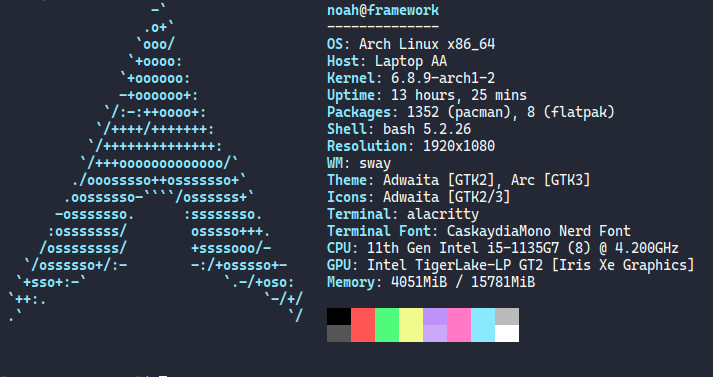
\includegraphics[width=0.7\textwidth]{../../res/neofetch.png}
        \caption{I use arch btw}
    \end{figure}
\end{frame}


\section{Some sprinkles!}

\begin{frame}
    \frametitle{ASCII Art to particles}

    \center
    You want to turn your favourite ASCII art into particles and see them CRASH?
    \newline
    \newline
    \newline
    Wait no more! 

\end{frame}


\begin{frame}
    \frametitle{ASCII Art to particles}

    \begin{figure}[H]
        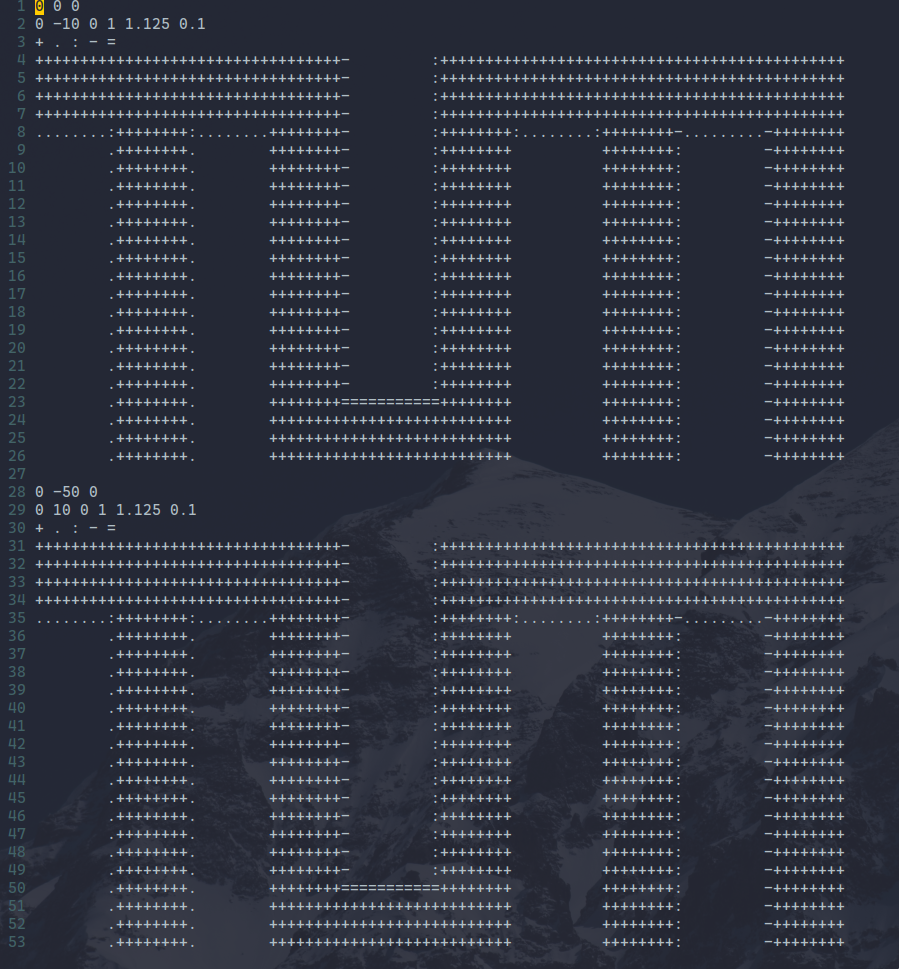
\includegraphics[width=0.43\textwidth]{/home/jimin/MolSim2/docs/res/tuminput}
    \end{figure}


\end{frame}


% Slides for References
\section{References}	
	\begin{thebibliography}
		\frame{
			\bibitem{StraPattern} https://refactoring.guru/design-patterns/strategy
		}
	\end{thebibliography}



\end{document}

